\chapter{Conclusions}
\label{chapter:conclusions}
\begin{music}
    \parindent10mm \instrumentnumber{1} \setstaffs1{1} 
    \generalmeter{\meterfrac64} \generalsignature{0}
    \startextract
		\notes \ql o \hl k \ql m \en \bar
              \notes \ql o \hl k \ql m \en \bar
              \notes  \Dqbl oq \ql p \ql n \Dqbl mn \en \bar
              \notes \ql o \ql k \Dqbl jl \ql k \en
    \zendextract
\end{music}
\epigraph{\textit{a childish mind will turn to noble ambition}}{Song of Time -- Ocarina of Time}

\section{Retrospectives}

In this thesis we explored the relationship between an organism phenotype and bifurcations in differential equations models seeking to model the organism behaviour. In the collaboration in synthetic biology in chapter \ref{chapter:double-exclusive}, the experimental design goals were to engineer a particular phenotypic behaviour of \emph{E. coli}. This amounted to designing particular bifurcations in the corresponding differential equation model. A gap in machine learning methods for differential equations that optimise with respect to targets directly in state space was identified, leading to the proposed method in Chapter \ref{chapter:inference}. We laid the foundations for methods that learn differential equation models that match qualitative behaviours and high-level constraints in state space. With this new method now in hand, we revisit how the collaboration in synthetic biology would have benefited and propose a \emph{Design-Learn} workflow that we argue would benefit any collaboration which designs phenotypes by iterative genetic manipulation of an organism \cite{Dalchau2018}. Differential equation models for an organism behaviour are not always available, as in the collaboration in immunology in chapter \ref{chapter:exploring}. We outlined the importance of interactive exploration and refinement of annotations of high-dimensional data clouds and built \emph{FlowAtlas.jl} to enable immunophenotyping across datasets with heterogeneous experimental designs. Our retrospectives are concluded with a vision of how methods from chapter \ref{chapter:exploring} can be used together with our proposed \emph{Design-Learn} workflow to organise and reduce different models of organisms whose behaviours can be experimentally captured with flow cytometry.

\subsection{A \emph{Design-Learn} workflow for synthetic biology}

One of the main insights from our collaboration in synthetic biology is the importance of the representation of the observed data in tuning the learned aspects of a hypothesis. The data representation must be invariant under  transformations that we do not want to learn. When engineering \emph{E. coli} we did not care about timescales or dynamical transients in the organisms response to experimental inputs. We also did not care about the exact concentrations of fluorescent proteins at steady state. The main concern was designing the shape of the bistable region in the experimental inputs.

This motivates processing flow cytometry data using basis function methods (Section \ref{section:basis-function-methods}) and running co-dimension two continuation methods to extract the limit curve that defines the separatrix between monostable and bistable regions in state space. The limit curve tells us where the steady state manifold folds, and can then be used as target data $\targets$ to infer parameters $\theta$ of some hypothesis $\rates$ using the method in Chapter \ref{chapter:inference}. Alternatively, one can optimise $\theta$ with respect to a geometric cost \eqref{eq:geometric-cost} that compares the field estimated from data $F$ to some parametrised hypothesis $\rates$. While kinetic information is ignored in this method, modes in the fluorescence distributions in the flow cytometry data define the locations of fixed points, and hence the shape of the steady state manifold. Whether design goals involve the whole shape of the steady state manifold or just its fold locations, a non-parametric representation $F$ of the data is required. Once the optimal parameters $\theta^*$ are obtained, the experimentalist can explore the neighbourhood of $\theta^*$ and see how they can change the bistable region, or whether they are close to another bifurcation which would produce a new phenotype. This can lead to new experiments that change the genotype $\theta^*+\Delta\theta$ in attempts to produce new phenotypes. Changes in genotype can involve promoter engineering for modulating transcription rates \cite{}, using degradation tags to change degradation rates \cite{} or ribosome binding site engineering for controlling translation \cite{}. The new data in turn can be used to refine the hypothesis; a summary of such a \emph{Design-Learn} pipeline is presented in Figure \ref{fig:deisgn-learn}.
\begin{Figure}
	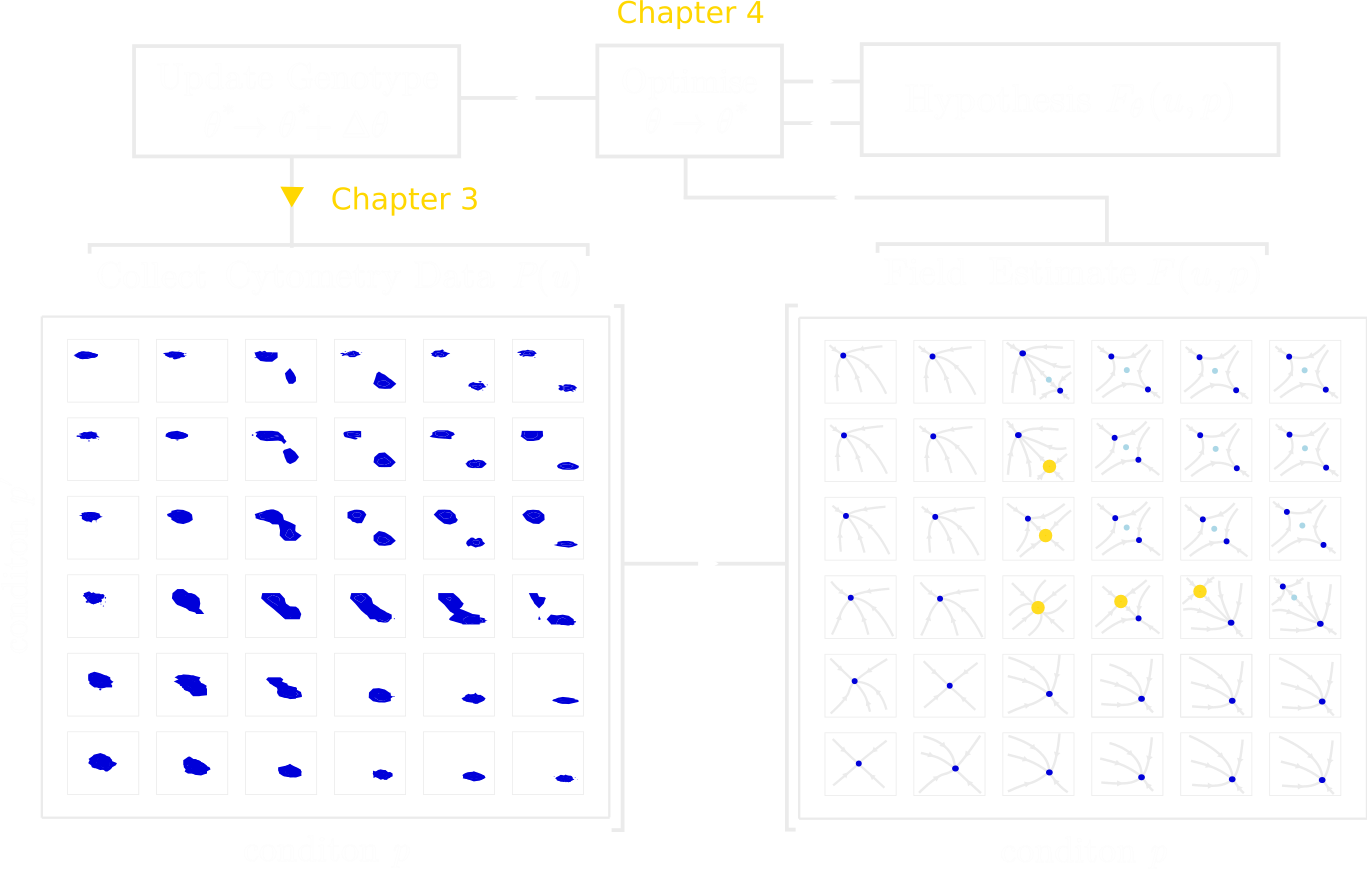
\includegraphics[width=\linewidth]{design-learn}
	\caption{Overview for a \emph{design-learn} workflow, developed in hindsight, for genetic design of the \emph{double exclusive reporter}. Non-parametric estimates of the field $F(u,p)$ yield state space geometry from cytometry data. A parametrised hypothesis $\rates(u,p)$ is then optimised against the data-driven state space geometry, to obtain optimal parameters $\theta^*$. The neighbourhood of $\theta^*$ is then investigated to decide which genetic modifications lead to improved designs, which are then tested with subsequent collection of more cytometry data.}
	\label{fig:deisgn-learn}
\end{Figure}
Approaches that do not require a non-parametric field $F$ to obtain target bifurcations $\targets$ involve quantifying the variance around clusters in the flow cytometry data. In the vicinity of bifurcations we expect certain scaling laws to emerge (Section \ref{section:fluctuations}) and localising bifurcations would require identifying such laws. A simple approach to this would be to localise cluster splitting, which was explored in Chapter \ref{chapter:double-exclusive} but never used to produce targets $\targets$ for optimisation. Accurate localisation of bifurcations using these methods require fine experimental sampling along the control condition $p$ and can ultimately be limited by intrinsic noise in the organism.

\subsection{Bifurcations \& model reduction}

\emph{E. coli} is a relatively simple organism whose genetic components can be individually modelled with biochemically reasonable assumptions and catalogued in a library of parts. This is not the case for the human immune system which was explored in chapter \ref{chapter:exploring}. Envisage how bifurcation theory, methods from chapter \ref{chapter:inference}, and \ref{chapter:exploring} can be combined to explore the space of hypotheses and reduced models for mechanisms in the immune system. A reduced model can be thought of in similar terms as a taylor expansion of a function around a specific point. The expansion has a reduced complexity compared to the original function and will have a finite region of validity around the point of expansion. Normal forms are in fact the lowest complexity expansions of a field in the vicinity of bifurcation points.

One of the simplest differential equation models of a flow cytometry dataset can be obtained by estimating a non-parametric field (Section \ref{section:basis-function-methods}) and then fitting normal forms around its bifurcations. The normal forms contain parameters that control the position and shape of bifurcations but are not biophysically interpretable. Models with biophysically interpretable parameters have larger complexity and a higher-dimensional state space. Despite this we find that bifurcating regimes cover finite regions of the parameter space. Moreover, these bifurcations happen along a centre manifold \cite{} whose dimension is equal to the number of vanishing eigenvalues. By expanding complex models in the vicinity of bifurcations along their centre manifolds, reduced models can be obtained. The reduced models in turn can be decomposed into normal forms. Following such a procedure, in principle, it is possible to establish a mapping between the biophysically interpretable parameters of the complex model and the normal form parameters that control the geometry of state space.

\begin{Figure}
	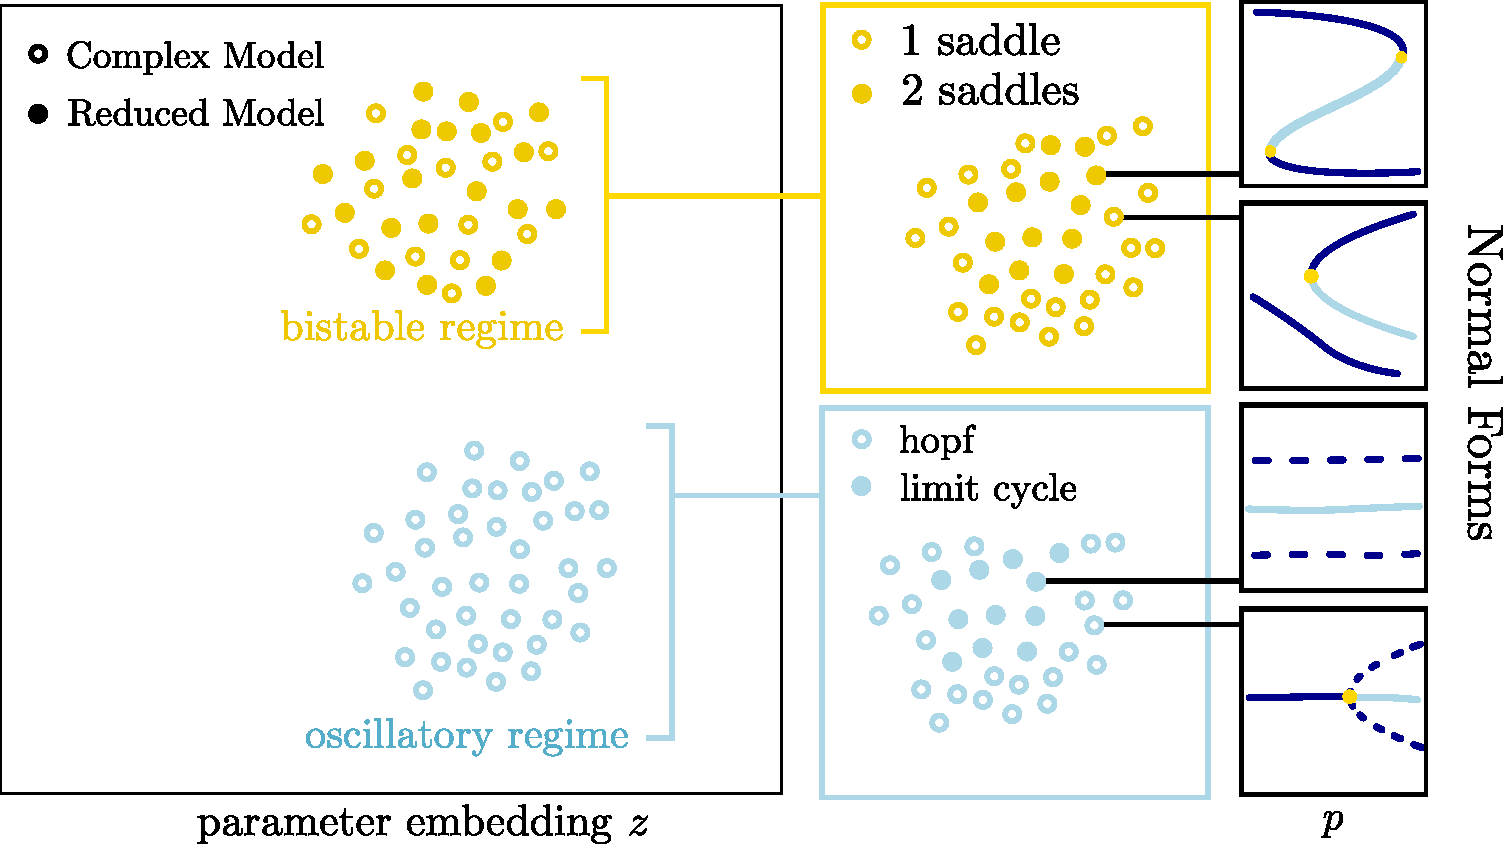
\includegraphics[width=\linewidth]{model-reduction}
	\caption{Overview of how \emph{FlowAtlas.jl} can be adapted to explore the space of models with respect to a given control condition $p$. The parameter embedding $z$ would align clusters of equivalent bifurcations in different models $\rates$, enabling the navigation of models of different complexity and discovery of reduced models}
	\label{fig:model-reduction}
\end{Figure}

Although we built \emph{FlowAtlas.jl} to navigate high-dimensional cytometry data, it can easily be re-applied to navigate any high-dimensional point clouds. Such point clouds emerge during optimal parameter estimation in chapter \ref{chapter:inference}. In this setting, each point represents a different set of parameters $\theta$ for the given model $\rates$ and each cluster represents a set of equally valid parameters that qualitatively match a given dataset $\targets$. Suppose there are many possible models $\rates$ with different dimensionality of $\theta$. How can we navigate the space of models with variable dimensionality? By embedding them in the same latent space, as we did with flow cytometry datasets with heterogeneous experimental designs in \emph{FlowAtlas.jl}. This embedding would have to map clusters that contain the same bifurcations for different models onto the same cluster in the latent space. Such a mapping would allow colouring and filtering a common embedding by model and bifurcation type, enabling navigation model space (Figure \ref{fig:model-reduction}) and discovering reduced models for complex flow cytometry datasets.

\section{Limitations}

\begin{itemize}
	\item Eigenvalue computation on steady state manifold
	\item Local gradient descent
\end{itemize}

\section{Future Work}

We now discuss future directions that would use this thesis as a starting point. In particular let us continue the discussion of limit cycle design with basis function methods (Section \ref{section:basis-function-methods}) and the extended bifurcation measure (Figure \ref{fig:hopf-measure}). We will see how in principle it is possible to design limit cycles whose sets are defined implicitly. We then conclude with how these approaches can be used to design spatially extended systems, in particular Turing bifurcations in self organised patterns and transitions to turbulence in fluid flows.

\subsection{Designing Limit Cycles}

Designing limit cycles requires two global constrains: a closed surface $\partial\Omega$ specified in the state space $u$ and an angular momentum field $\omega(u)$ that gives rise to circulating trajectories along the surface $\partial\Omega$. Basis function methods (Section \ref{section:basis-function-methods}) naturally give rise to an unstable focus that pushes trajectories towards the limit cycle from within the surface $\partial\Omega$. We can perform gradient descent against the geometric cost function \eqref{eq:geometric-cost} using the non-parametric field in the vicinity of the limit cycle as a target. This designs the shape of the limit cycle, but not the bifurcations that created it. By combining the geometric cost \eqref{eq:geometric-cost} and the bifurcation measure (Figure \ref{fig:hopf-measure}) we can simultaneously design the shape of the limit cycle as well as the bifurcations around it. 

\begin{Figure}
	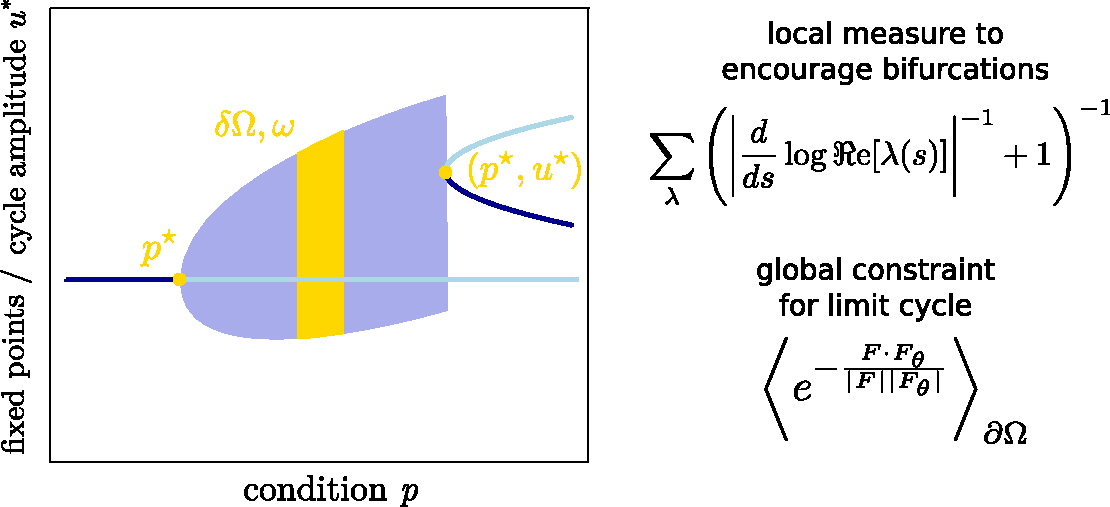
\includegraphics[width=9cm]{design-limit-cycles}
	\caption{Using global constraints $\partial\Omega,\omega$ with basis functions in state space $u$ and local constraints at $p^\star,u^\star$ can help design global bifurcations of limit cycles}
	\label{fig:design-limit-cycles}
\end{Figure}

As an example, suppose we would like to design a limit cycle that emerges from a local Hopf bifurcation from the left and disappears in a global infinite period bifurcation from the right  (Figure \ref{fig:design-limit-cycles}). In principle we could use the bifurcation measure (Figure \ref{fig:hopf-measure}) to encourage Jacobian eigenvalues crossing the imaginary axis $\Real[\lambda]=0$ at local points $(p^\star,u^\star)$ and hope that a limit cycle appears in between them. However this could merely result in a model two saddle node bifurcations, yielding a bistable region in between the two points $p^\star$. In order to guarantee a limit cycle we specify create a non-parametric field $F$ with global constraints $\partial\Omega,\omega$ and include it in a geometric cost. Note that we only need to evaluate the model to be optimised $\rates$ in the vicinity of the limit set $\partial\Omega$ and in principle this can be done sparsely so save compute time. The key takeaway is that by combining local constrains via Jacobian eigenvalues and global constraints via basis function in state spaces, it is possible to design global bifurcations (Section \ref{section:global-bifurcations}).

\subsection{Spatially Extended Systems}
